\subsection{Repeated train/pool splits}\label{sec:splits}

All earlier results use one train/pool split and one set of nine fitted models per setting. To measure how much the efficiency depends on the split, we repeated the main study for the six largest settings (Adult with sex and with race as the group, Bank marketing, credit-card default, MAGIC and Electricity; pools of $7608$ to $19537$ instances) on three new splits, with seeds $1$, $2$ and $3$. For each split the nine models were refitted on the new $60\%$ training part (the learners' own random seeds were not changed, so the variation comes from the data split and the refit), the pool is the new $40\%$ held-out part, and the protocol of Section~\ref{sec:empirical} was run for SRS, GROUP, PATTERN and PATTERN-DIF with $L\in\{500,1000\}$ and $R=100$ replicates per cell. The original split (seed $0$, $R=200$) is included as the fourth value. The code is \texttt{experiments/label\_efficiency\_splits.py}; the numbers are in \texttt{results/label\_efficiency\_splits.json} and \texttt{results/label\_\allowbreak efficiency\_\allowbreak splits\_\allowbreak summary.json}. Efficiency is defined as before, the median over contrasts of the ratio of mean squared errors against SRS, computed on the pool of each split.

\begin{table}[t]
\centering\small
\caption{Efficiency of PATTERN-DIF against SRS (ratio of mean squared errors) on four train/pool splits. Split 0 is the original one. Mean, standard deviation and range are over the four splits. The last rows give the median over the six settings. Source: \texttt{results/label\_efficiency\_splits.json}.}\label{tab:split-main}
\begin{tabular}{lrrrrrrrr}\toprule
Setting & $L$ & split 0 & split 1 & split 2 & split 3 & Mean & SD & Range \\\midrule
Adult (sex) & 500 & 6.8 & 7.8 & 6.8 & 8.1 & 7.4 & 0.7 & 6.8--8.1 \\
 & 1000 & 7.8 & 7.3 & 7.2 & 7.8 & 7.5 & 0.3 & 7.2--7.8 \\
\addlinespace
Adult (race) & 500 & 12.4 & 10.6 & 12.8 & 14.6 & 12.6 & 1.6 & 10.6--14.6 \\
 & 1000 & 14.7 & 14.9 & 16.4 & 15.6 & 15.4 & 0.8 & 14.7--16.4 \\
\addlinespace
Bank marketing & 500 & 12.1 & 11.6 & 12.4 & 11.6 & 11.9 & 0.4 & 11.6--12.4 \\
 & 1000 & 15.0 & 15.2 & 13.2 & 12.7 & 14.0 & 1.2 & 12.7--15.2 \\
\addlinespace
Credit card & 500 & 5.3 & 5.6 & 6.1 & 6.7 & 5.9 & 0.6 & 5.3--6.7 \\
 & 1000 & 6.0 & 6.5 & 7.9 & 6.7 & 6.8 & 0.8 & 6.0--7.9 \\
\addlinespace
MAGIC & 500 & 4.8 & 4.5 & 5.4 & 5.0 & 4.9 & 0.4 & 4.5--5.4 \\
 & 1000 & 5.4 & 5.2 & 5.2 & 5.8 & 5.4 & 0.3 & 5.2--5.8 \\
\addlinespace
Electricity & 500 & 4.5 & 4.3 & 4.2 & 4.3 & 4.3 & 0.1 & 4.2--4.5 \\
 & 1000 & 5.0 & 5.3 & 4.5 & 4.9 & 4.9 & 0.3 & 4.5--5.3 \\
\addlinespace
Median over settings & 500 & 6.0 & 6.7 & 6.5 & 7.4 & \multicolumn{3}{c}{} \\
Median over settings & 1000 & 6.9 & 6.9 & 7.6 & 7.3 & \multicolumn{3}{c}{} \\
\bottomrule\end{tabular}

\end{table}

\begin{figure}[t]
\centering
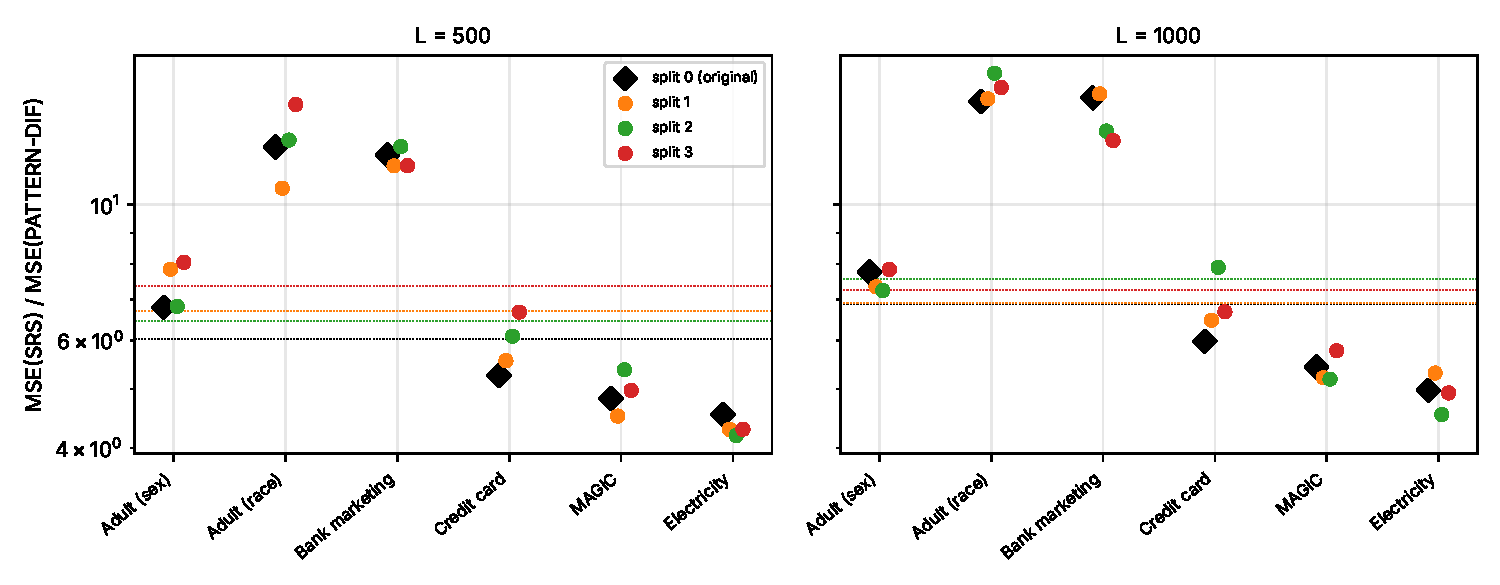
\includegraphics[width=\textwidth]{figures/splits_efficiency}
\caption{Efficiency of PATTERN-DIF against SRS by setting and split. The diamond is the original split. Dotted lines are the medians over the six settings for each split.}\label{fig:split-eff}
\end{figure}

Table~\ref{tab:split-main} and Figure~\ref{fig:split-eff} show that the efficiency is stable across splits relative to its variation across settings, which ranges from $4.9$ (Electricity, mean over the four splits) to $15.4$ (Adult with race) at $L=1000$. The median over settings of the coefficient of variation across the four splits is $0.07$ and the median ratio of the largest to the smallest split value is $1.18$. The largest spreads are Adult (race) at $L=500$ (from $10.6$ to $14.6$) and Credit card at $L=1000$ ($6.0$ to $7.9$). Part of this spread is Monte Carlo error, since each value rests on $100$ replicates ($200$ for split $0$). Adult (race) and Bank have the highest efficiency and Electricity and MAGIC the lowest in every split and at both budgets. The efficiency of PATTERN-DIF is at least $4.2$ in all $48$ cell-split values.

The median over the six settings is $6.0$, $6.7$, $6.5$ and $7.4$ at $L=500$ for splits $0$ to $3$, and $6.9$, $6.9$, $7.6$ and $7.3$ at $L=1000$. The original split gives the lowest median of the four at both budgets (at $L=1000$ only marginally below split~1), so the choice of split does not flatter the headline numbers of the main study in these settings. Pooling the four splits, the median is $6.7$ at $L=500$ and $7.3$ at $L=1000$ against $6.0$ and $6.9$ for split $0$ alone, a difference of at most about $12\%$ on a factor of 6 to 7. Coverage is unaffected: the mean coverage of the PATTERN-DIF intervals is $0.948$ to $0.951$ on every split ($0.950$ overall), against $0.939$ to $0.941$ for SRS with the plug-in estimator. The worst contrast in any split has coverage $0.84$ to $0.88$ for PATTERN-DIF; with $100$ replicates per cell the Monte Carlo standard error of one coverage is $0.02$, so these worst values are partly noise.

These results have three limits. Four splits in total (three new) are far fewer than the $20$ that a full study of between-split variation would use, so the spread in Table~\ref{tab:split-main} is a rough indication only. Only the six largest settings were repeated, so the median over all eleven settings of the main study is not recomputed. The nine models share the same families in every split, and the splits do not change the learner seeds or the groups, so variation from other hyperparameters or model families is not covered.
